\section{Technical documentation}

In this chapter, the a tutorial for setting up the simulation and the analysis of the IDEA detector is described. More information on the FCC software is available on the \href{http://fccsw.web.cern.ch/fccsw/}{FCCSW webpage}~\cite{FCCSW}.

\subsection{Installation of FCCSW from GitHub}

First, fork the FCCSW repository on \href{https://github.com/HEP-FCC/FCCSW}{GitHub}. Log in to \textsc{lxplus SLC6} and clone your fork of the project.

\begin{lstlisting}[language=bash,caption={Clone your fork of the FCCSW repository.}]
  git clone https://github.com/[your-github-username]/FCCSW.git
  cd FCCSW
\end{lstlisting}

Make sure to correctly set remote for the GitHub repository using the following \href{https://help.github.com/en/articles/configuring-a-remote-for-a-fork}{guide}\footnote{\href{https://help.github.com/en/articles/configuring-a-remote-for-a-fork}{https://help.github.com/en/articles/configuring-a-remote-for-a-fork}}. To sync your fork with the upstream repository use the instructions given in this \href{https://help.github.com/en/articles/syncing-a-fork}{guide}\footnote{\href{https://help.github.com/en/articles/syncing-a-fork}{https://help.github.com/en/articles/syncing-a-fork}}.

Setup the environment in order to build or use the software.
\begin{lstlisting}[language=bash,caption={Setup the environment and compile.}]
  source ./init.sh
  make -j 12
\end{lstlisting}

\subsection{Running FCCSW}

In order to visualise the geometry of the FCCeeIDEA detector run the following command and the display is shown in \cref{fig_sim_vis}.

\begin{lstlisting}[language=bash,caption={Visualise the full geometry of the FCCeeIDEA detector.}]
./run geoDisplay -compact \
  Detector/DetFCCeeIDEA/compact/FCCee_DectEmptyMaster.xml \
  Detector/DetFCCeeIDEA/compact/FCCee_DectMaster.xml
\end{lstlisting}

\begin{figure}[!t]
\centering
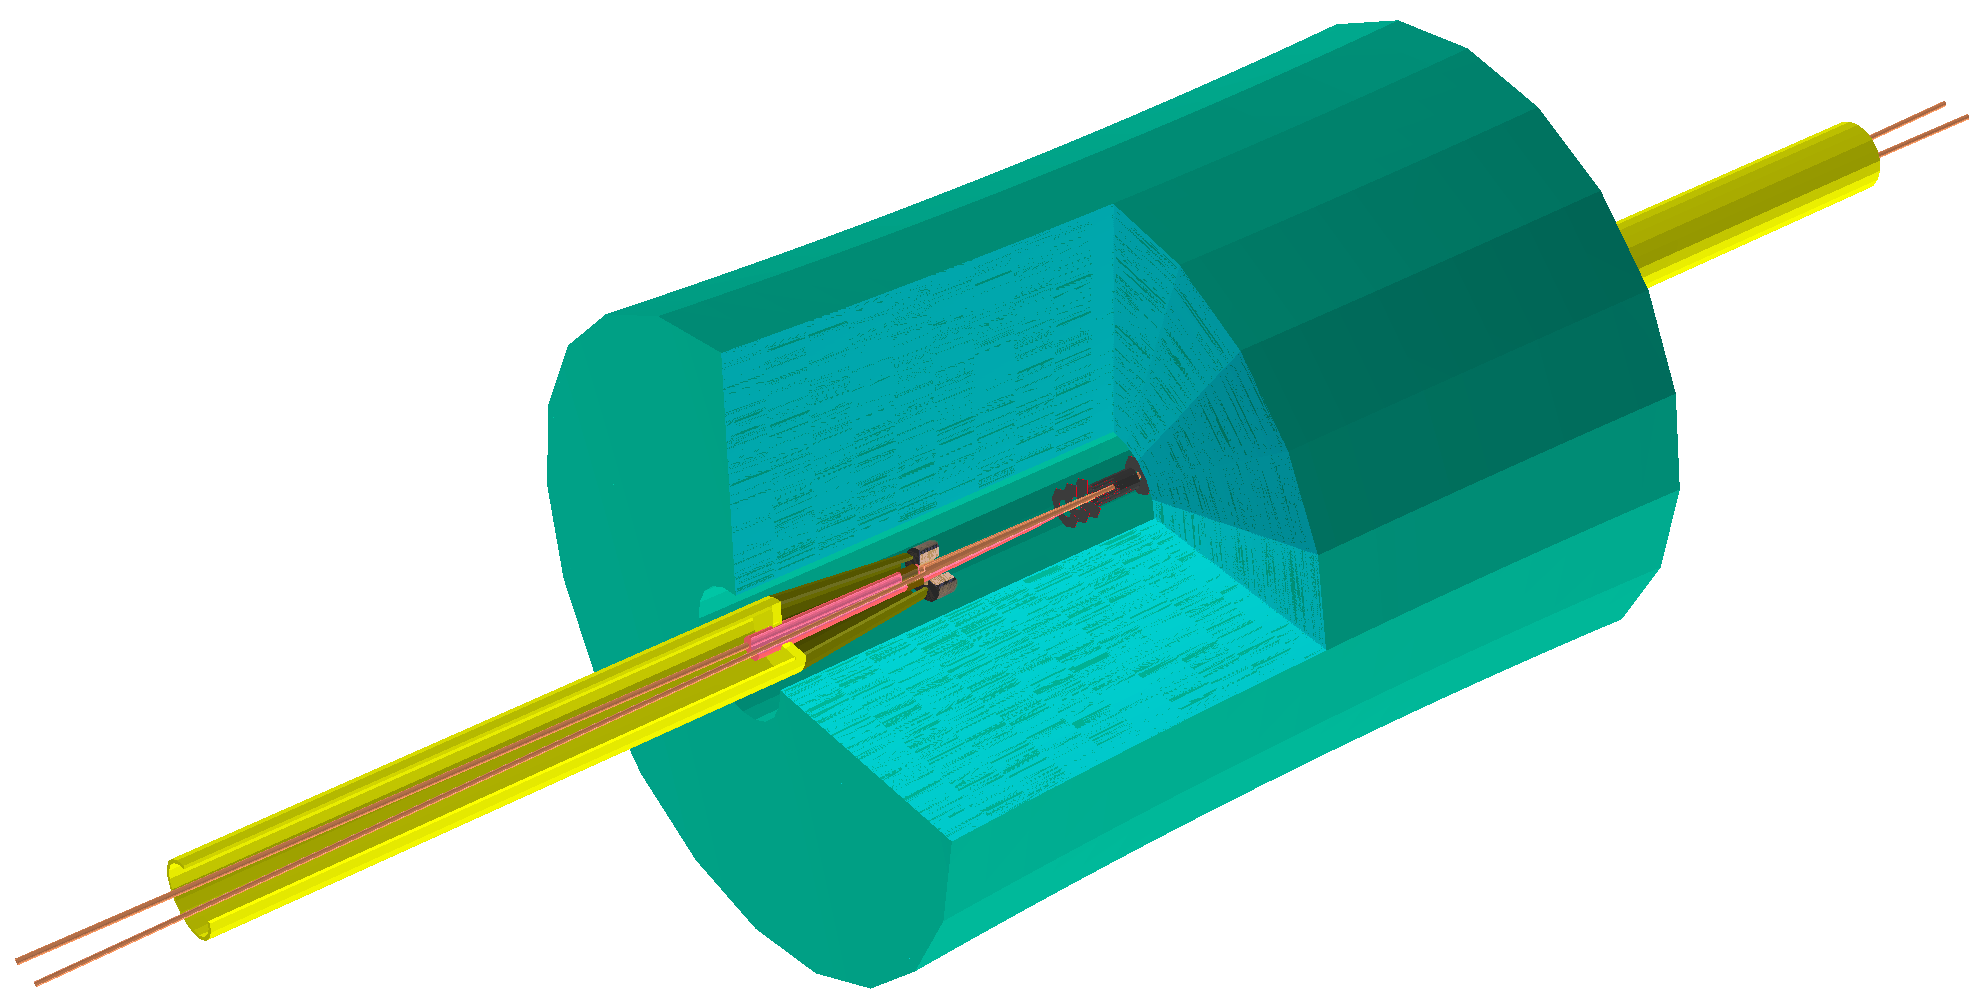
\includegraphics[width=0.8\textwidth]{figures/FCCeeIDEA_IR}

\caption{Visualisation of the FCCeeIDEA detector using FCCSW.}
\label{fig_sim_vis}
\end{figure}

The following script is used to run a simulation using particle gun from \textsc{Geant4}. The output is written in a PODIO file. The output contains the energy deposits calculated by \textsc{Geant4} at each \textsc{G4Step}.

\begin{lstlisting}[language=bash,caption={Particle gun simulation.}]
./run fccrun.py Examples/options/geant_fullsim_fccee_pgun.py
\end{lstlisting}

\subsection{Hit Reconstruction}

The hits (or energy deposits calculated at each \textsc{G4Step}) are then drifted to the corresponding wire. This step, outputs a ROOT file containing the wires hit (cellID, layerID and wireID), the Monte Carlo Truth positions, the distance of the closest approach of the track to the wire hit.

\begin{lstlisting}[language=bash,caption={Reconstruction of the simulated hits for the drift chamber.}]
  ./run fccrun.py \
  Reconstruction/RecDriftChamber/tests/options/mergeHits.py
\end{lstlisting}
